\documentclass[
	12pt, % Font size
	a4paper, % Paper size
	oneside, % One-sided document
]{report}

% Set the PDF version for LuaTeX
\usepackage{luacode}
\begin{luacode}
  pdf.setminorversion(6)
\end{luacode}

% Packages
\usepackage[english]{babel} % Set document language
\usepackage{pdfpages} % Include PDF files
\usepackage[utf8]{inputenc} % UTF-8 encoding (for umlauts etc.)
\usepackage[T1]{fontenc} % correct hyphenation
\usepackage{csquotes} % correct quotation marks
\usepackage{lmodern} % Computer Modern fonts
\usepackage{microtype} % better typesetting results (avoids underfull / overfull hboxes)
\usepackage{graphicx} % adding graphics
\usepackage{units} % typesetting units, e.g. \unit[10]{MB} and \unitfrac[100]{Mbit}{s}
\usepackage{booktabs} % publication quality tables
\usepackage{titlesec} % Customize chapter and section headings
\usepackage{setspace} % Set line spacing
\usepackage{geometry} % Set page margins
\usepackage{subcaption}
\usepackage{float}
\usepackage[
	backend=bibtex,
	style=numeric-comp,
	maxcitenames=2,
	natbib=true,
	sorting=none
]{biblatex} % Bibliography

% Bibliography
\addbibresource{literature.bib}

% Title page
\title{Title of Your Thesis}
\author{Til Mohr}
\date{\today}

% Document
\begin{document}

% Title page
\maketitle

% Eidesstattliche Versicherung
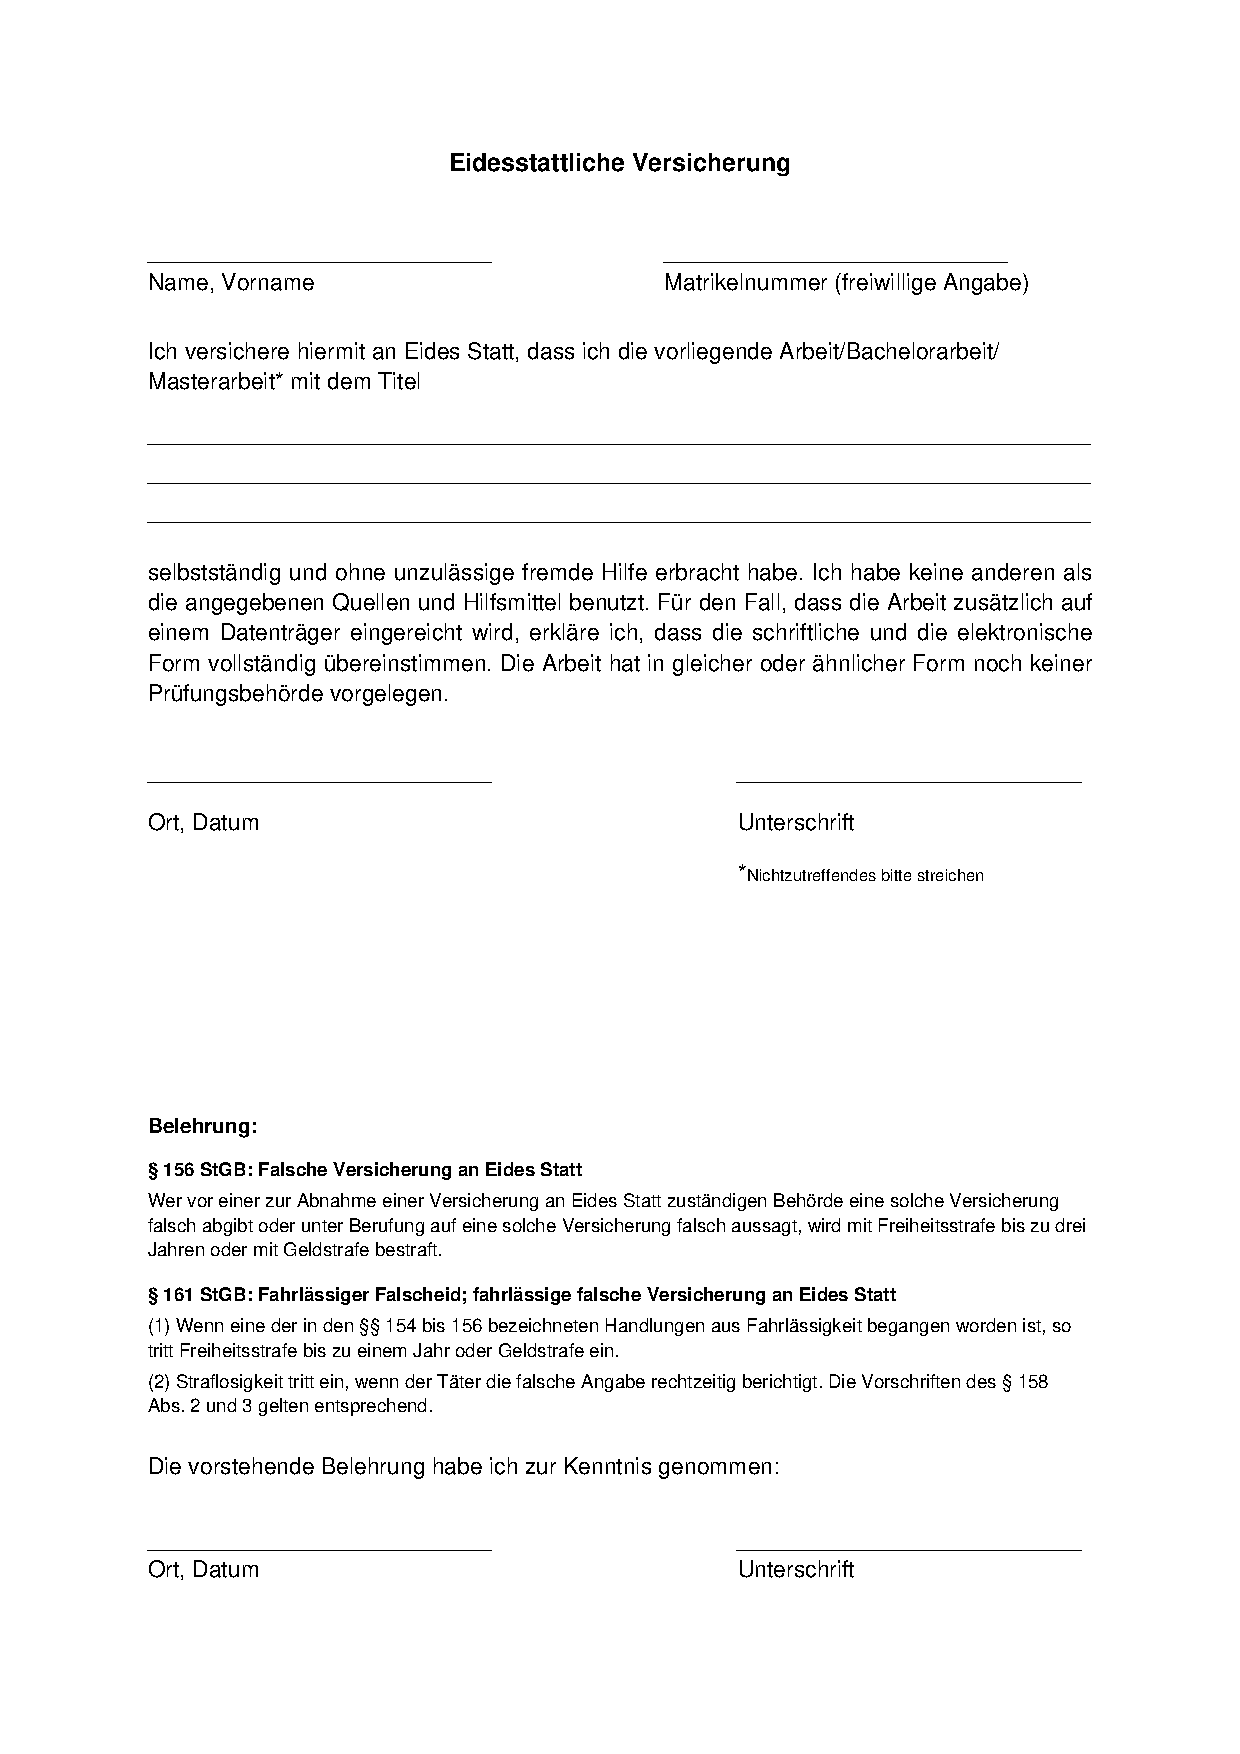
\includepdf{Formular_Eidesstattliche_Versicherung.pdf}

% Abstract
\begin{abstract}
This is the abstract of your thesis.
\end{abstract}

% Table of contents
\tableofcontents

% Chapters
\chapter{Introduction}
\section{Background}

\chapter{Literature Review}
\section{Previous Studies}

% Conclusion
\chapter{Conclusion}

% References
\begin{thebibliography}{9}
\bibitem{ref1} Author. \textit{Title of the Reference}. Publisher, Year.
\end{thebibliography}

\end{document}
% Chapters
\chapter{Methodology}
\section{Research Design}

\chapter{Results}
\section{Data Analysis}

\chapter{Discussion}

% Appendix
\appendix
\chapter{Additional Information}

% End of document
\end{document}